\chapter{INCIDENT RADIATION FIELD SHAPE}
% !TEX root = hazy1.tex
\label{sec:IncidentContinuumShape}

\section{Overview}

The spectral energy distribution (SED) of the
incident radiation field should be specified
between the energies of \emm\ ($\lambda \approx$ \emmcm )
and \egamrymev \ $\approx$ \egamry .
The low-energy region is important for Compton cooling,
photoionization
from excited states of the elements, free-free heating, H$^-$ heating,
and grain heating.
The high-energy portion is important for Auger and secondary
ionization, Compton heating, and pair production.
Energies greater than
100 MeV are not generally important since the Klein - Nishina
electron-scattering cross section is small.
\Cloudy\ will complain, but compute
the model if possible, if the
incident radiation field is not specified over the full energy range.
An intensity of zero will be assumed for missing portions of the
incident radiation field.

The \cdTerm{plasma frequency}, given by
\begin{equation}
\nu _{pl}  = \left( {\frac{{n_e q_e^2 }}{{\pi \,m_e }}} \right)^{1/2}  =
8.978 \times 10^3 \,n_e^{1/2} \;s^{ - 1}  = 2.729 \times 10^{ - 12}
\;n_e^{1/2} \;{\mathrm{Ryd}},% (15)
\end{equation}
will move into the energy range considered by the code if the electron
density is higher than $\sim 10^7 \mathrm{cm}^{-3}$.
The incident radiation field below the
plasma frequency is totally reflected and does not enter the slab.
The code will generate a comment if the plasma frequency occurs within
the energy grid.

\emph{It is important to plot the incident radiation
field using the output of the
\cdCommand{save continuum} command to make sure the SED has the expected shape.}
It is easy to make a mistake in converting between $f_\nu$, $f_\lambda$,
$\nu f_\nu$, and $\lambda f_\lambda$ when deriving the SED.
The \cdCommand{save continuum} command will report the SED in 
$\nu f_\nu$ or $\lambda f_\lambda$ units (the two are equivalent).

\subsection{Isotropic and beamed continua}
Most radiation fields are assumed to strike the cloud as a
single-directional beam.
The beam is assumed to enter the slab normal to
the surface, unless this is changed with the
\cdCommand{illumination angle} command.
Other commands, including
\cdCommand{background}, \cdCommand{CMB},
\cdCommand{table HM96}, \cdCommand{table HM05},
\cdCommand{table HM12}, and \cdCommand{table ISM},
generate continua that are isotropic.
Each shape command will indicate whether the SED is isotropic or beamed.

Many spectrometers will automatically remove isotropic emission while
conducting an observation.  Some isotropic continua, especially the CMB at
radio wavelengths, will dominate over local emission.
The radiation field used in the calculation is reported by default, although
there are two commands that will suppress isotropic emission.
The \cdCommand{save continuum} command,
section \ref{sec:CommandSaveContinuum}, includes a \cdCommand{no isotropic}
option, described in section \ref{sec:save_cont_no_isotropic_option}, to suppress
isotropic emission in that file.
The \cdCommand{no isotropic continua report} command described
in section \ref{sec:no_isotropic_continua} will suppress
Isotropic emission in both \cdCommand{save continuum}  files
and the continuum bands described in
Section~\ref{Hazy2-sec:Radiation-field-integrated-over-wavelengths}
\cdSectionTitle{\refname{Hazy2-sec:Radiation-field-integrated-over-wavelengths}}.


\section{AGN T =1.5e5 k, a(ox) = -1.4, a(uv)=-0.5 a(x)=-1}

This produces a multi-component continuum similar to that observed in
typical Active Galactic Nucleus (AGN).
An example is shown in Figure \ref{fig:agncon}.
The ``Big Bump'' component, peaking at $\approx 1$ Ryd,
is a rising power law with
a high-energy exponential cutoff.
It is parameterized by the temperature
of the bump, the first argument on the command line.
It is interpreted
as the log of the temperature if it is less than or equal to 10 and the
linear temperature otherwise.
The temperature of the bump can by optimized by using the \cdCommand{vary} keyword.
The second parameter is the X-ray to UV ratio
$\alpha_{ox}$.
Note that there
is no implicit negative sign in this exponent; typical AGN have
$\alpha_{ox} \sim
-1.4$, (\citealp{Zamorani1981}).
The third (optional) argument is the
low-energy slope of the Big Bump continuum,
with the default $\alpha_{uv} = -0.5$
(\citealp{Elvis1994}; \citealp{Francis1993}).
The last argument is the slope of the
X-ray component with the default $\alpha_x = -1$.
Optional parameters can be omitted
from right to left.

\begin{figure}
\centering
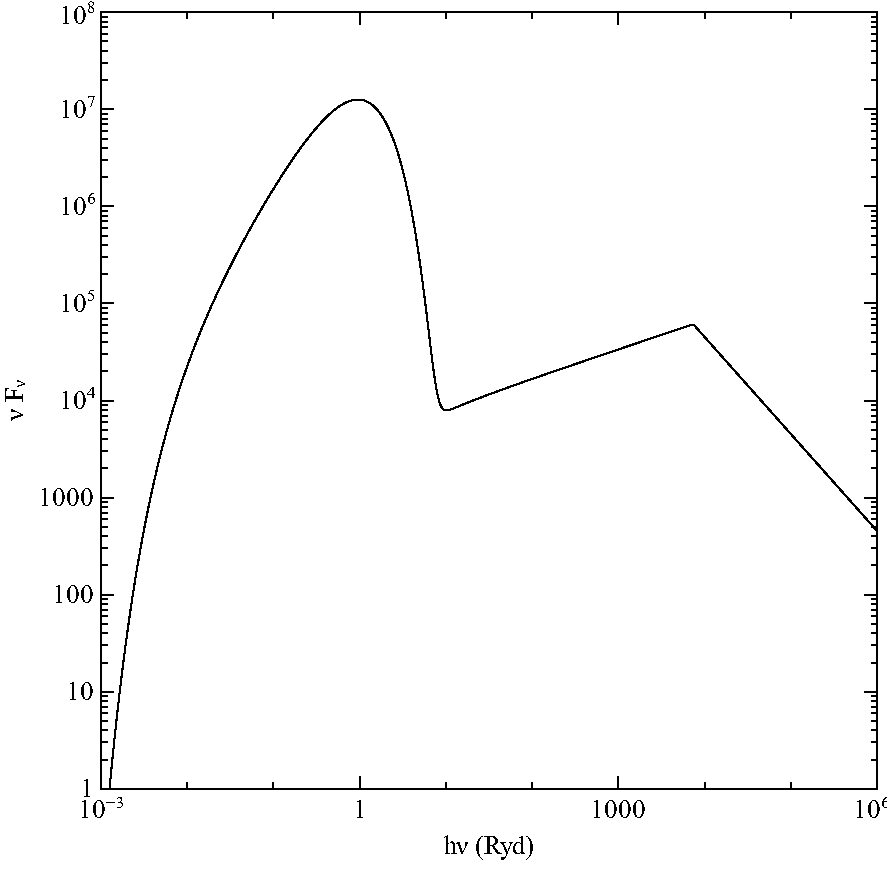
\includegraphics[scale=0.75]{AGNCON}
\caption[AGN SED]{\label{fig:agncon}The continuum produced by the
\cdCommand{AGN} continuum command.
The Big Bump peaks at $\approx1$~Ryd,
while the X-ray power law dominates at high energies.
The two components are normalized by the second parameter, the value of
$\alpha_{ox}$.}
\end{figure}

The full continuum is the sum of two components,
as in equation \ref{eqn:agncon}:

\begin{equation}
\label{eqn:agncon}
f_\nu   = \nu ^{\alpha _{uv} } \exp \left( { - h\nu /kT_{BB} } \right)\exp
\left( { - kT_{IR} /h\nu } \right)\; + a\nu ^{\alpha _x }. % (16)
\end{equation}
The coefficient $a$ is adjusted to produce the
correct $\alpha_{ox}$ for the case where
the Big Bump does not contribute to the emission at 2~keV.
If the bump
is very hot then it may contribute to the X-rays as well and
the resulting
continuum will have a more negative $\alpha_{ox}$ than specified.
The X-ray power
law is only added for energies greater than 0.1 Ryd to prevent
it from
extending into the infrared, where a power law of this slope
would produce
\emph{very} strong free-free heating.
The Big Bump component is assumed to have
an infrared exponential cutoff at $kT_{IR} = 0.01 \mathrm{Ryd}$.

The last term in equation \ref{eqn:agncon} is not extrapolated
below 1.36 eV or above 100 keV.
Below 1.36 eV the last term is simply set to zero (the bump
dominates for these energies).
Above 100 keV the continuum is assumed to
fall off as $v^{-2}$.

The exponential cutoff in the low-energy end of the Big Bump will cause
the incident continuum to have zero intensity at very long wavelengths.
The code will complain since a zero incident continuum is unphysical, but
the model will be computed.
You can prevent the continuum from going to
zero by including the cosmic background with the
\cdCommand{background} command or with the \cdCommand{CMB} command.

We used this command to generate the continuum used in a large atlas
of BLR line intensities (\citealp{KoristaBaldwin1997}).
The specific parameters
needed to reproduce that continuum are
\cdCommand{AGN 6.00 -1.40 -0.50 -1.0}.  Only
Kirk Korista can remember all these numbers and the parameters were not
explicitly given in the original paper in the format used by the code.
The \cdCommand{kirk} option on the \cdCommand{AGN} command will
generate that continuum.
It is fairly
similar to the \citet{Mathews1987} continuum but there is
much greater
flexibility in changing its details.

\section{Background, z=1.825, [f=100; no CMB]}

This specifies a radiation field shape and intensity
chosen to mimic the cosmic
radio to X-ray background (\citealp{Ostriker1983}, \citealp{Ikeuchi1986}, and \citealp{Vedel1994}).
Their ultraviolet
continuum shape is an $\alpha = -1$ power-law, with a mean intensity
$J_\nu$ at 912\AA\ given~by
\begin{equation}
4\,\pi \;J_\nu  \left( {912{\mathrm{{\AA}}}} \right) = 4\,\pi \, \times 10^{
- 21} \left( {\frac{{1 + z}}{{3.5}}} \right)^4 \quad f [\mathrm{erg\, Hz}^{-1}
\mathrm{cm}^{-2} \, \mathrm{s}^{-1}]
\end{equation}
where $z$ is the redshift and $f$ an optional scale factor entered as
the second parameter.
Its default value is $f = 1$, and $z = 0$ (i.e., now) is assumed
if no redshift is entered.
Judging from \citet{Bechtold1987}, \citet{Bajtlik1988}, and \citet{Vedel1994},
$f$ is confidently known to be within an order of magnitude of unity.

This command specifies \emph{both} the shape and intensity
of the incident radiation field.
It is important that any previously occurring ordered pairs of shape and
intensity commands be complete before this command is given.

Cosmic microwave background radiation is included in the generated
background.
This radiation field is assumed to be a blackbody radiation
field, in strict thermodynamic equilibrium, with temperature given~by
\begin{equation}
T_{CMB}  = T_o \left( {1 + z} \right)\; [\mathrm{K}]% (18)
\end{equation}
where the redshift dependence is from \citet{Peebles1971} and the present
temperature of the background is assumed to be $T_o = 2.725 \pm 0.002$K
(\citealp{Mather1999}; \citealp{Wilkinson1987}).
This background can be an important source
of Compton cooling for low-density clouds.
If the optional keyword
\cdCommand{no CMB}
appears on the line then the CMB background will not be included.
The CMB can be specified independently with
the \cdCommand{CMB} command.

The \cdCommand{table HM96} command uses a more sophisticated
form of the energetic continuum, but only at a redshift of $z = 2$.
The \cdCommand{table HM05} and \cdCommand{table HM12}
commands work at any redshift.

This command does not add the cosmic-ray background.
This should be
included if the simulation is to extend into molecular gas and is done
separately with the \cdCommand{cosmic ray} command.

This radiation field is assumed to be isotropic rather than beamed.

\section{Blackbody t=e5 K [linear, log, luminosity]}

The continuum will be a blackbody with temperature (K) given by the
number.
The temperature may be entered directly or as a log.
The number
is assumed to be a log if it is less than or equal to 10 and linear if
greater than 10.
The keywords \cdCommand{log} and \cdCommand{linear} will override
this default
and force the interpretation of the numbers to be either a log or linear.
Embedded commas can improve readability, such~as
\begin{verbatim}
black body, Temp = 1e6 K
\end{verbatim}
which is equivalent to
\begin{verbatim}
black 1000000
\end{verbatim}
or
\begin{verbatim}
black body t=6  .
\end{verbatim}

\subsection{Blackbody, t = 1e5 K, disk = 1e3 K}

This command produces a multi-color blackbody as if due to an accretion disk  with
inner and outer temperatures $T_{in}$ and $T_{out}$ as in \citet{Mitsuda1984}.  
The temperatures can be in either order; the code will automatically take the 
greater temperature as $T_{in}$.  

Neither the luminosity nor the intensity is set by this command.

\subsection{Peter Martin's blackbody luminosity options}

The luminosity of the black body can be specified with command-line
options added by P.G. Martin.
If the luminosity is specified
with any of these options then it must not also be specified with another
luminosity command for this radiation field.
The keywords that can appear
on the line are given in the following subsections.

\subsection{Blackbody 5, luminosity = 38.   }

If the keyword \cdCommand{luminosity} appears then the second number
is the log of
the \emph{total} luminosity (erg s$^{-1}$) of the black body, $4\pi \,R_{star}^2 \sigma T_{eff}^4 $
(this number is interpreted as a log even when the keyword \cdCommand{linear} appears on the line).
This example would be a 10$^5$~K planetary nebula nucleus at the Eddington
limit.

This is a luminosity command.

\subsection{Blackbody 5, radius = 10.  }

The log of the radius (in cm) of the blackbody $R_{star}$
is used to set the
total luminosity when the keyword \cdCommand{radius} appears
(this number is interpreted as a log even when the keyword \cdCommand{linear} appears on the line).
The total luminosity
is $4\pi \,R_{star}^2 \sigma T_{eff}^4 $.
This example is also typical of a planetary nebula nucleus.

This is a luminosity command.

\subsection{Blackbody 5e4 K, energy density = 500K.  }

The energy density of the blackbody radiation field, expressed as the
equivalent blackbody temperature $T_u$ in degrees Kelvin,
is used to set the
luminosity when the \cdCommand{energy density} keyword appears
anywhere on the line.
The energy-density temperature is defined from Stefan's law and the energy
density of the radiation field $u$~[erg cm$^{-3}$]:
\begin{equation}
T_u  \equiv \left( {\frac{u}{a}} \right)^{1/4}  [\mathrm{K}]% (19)
\end{equation}
where $a$ is the Stefan's radiation density constant.

Both temperatures are interpreted as logs if they are less than or equal
to 10 or the keyword \cdCommand{log} appears, and linear otherwise.  They will be interpreted as the linear
temperature rather than as a log if the keyword \cdCommand{linear} appears.  Note that
if the \cdCommand{linear} key is used then both temperatures are interpreted as linear.
Similarly, if the keyword \cdCommand{log} appears, both temperatures are interpreted as log.
Note also that the cosmic background radiation should also be included if
$T_u\le 2.725 (1+z) K$.
\Cloudy\ will complain, but compute the model, if the
energy density of the incident continuum corresponds to a temperature less
than the present energy-density temperature of the universe.

This is an intensity command.

\subsection{Blackbody, t = 5e4 K, STE  }

The keyword \cdCommand{STE}\footnote{The keyword was \cdCommand{LTE} before version 96 of the code.  It was changed
to \cdCommand{STE} to better reflect the fact that this condition corresponds to strict
thermodynamic equilibrium.
The code will continue to accept the \cdCommand{LTE} keyword
for the foreseeable future.}
(note that a space must appear before ``STE'') with no second number is
equivalent to the \cdCommand{energy density} option with $T_u$ set
to the color temperature
of the radiation field.
This is a quick way to check that ionization and
level populations go to strict thermodynamic equilibrium in the high
radiation-density limit.

This is an intensity command.

\subsection{Blackbody, t = 1e5 K, dilution factor = -14}

Here the second parameter is the \cdTerm{dilution factor}
\cdTerm{W} defined as
\begin{equation}
W \equiv \frac{{J_\nu  }}{{B_\nu  }} \approx \frac{{\pi \,R_{star}^2
}}{{4\,\pi \;r_o^2 }},% (20)
\end{equation}
where $R_{star}$ is the radius of the star and $r_o$ is the separation
between the illuminated face of the cloud and the center of the star.
The approximation
on the RHS assumes that $R_{star} \ll r_o$.
The dilution factor can be entered
either directly or as a log. Any number $> 0$ will be interpreted as
linear, while any number $\leq 0$ will be interpreted as log.
The example above is a rough approximation of the radiation field within
a typical planetary nebula.

This is an intensity command.

\section{Bremsstrahlung, temp = 8}

The incident radiation field will be optically thin pure hydrogen bremsstrahlung
emission.
The shape is given~by
\begin{equation}
f_\nu   \propto \nu ^{ - 0.2} \,\exp \left( { - h\,\nu /kT} \right)\quad
[\mathrm{erg\, cm}^{-2} \mathrm{s}^{-1} \mathrm{Hz}^{-1}]. %(21)
\end{equation}
The argument is assumed to be the log of the temperature if it is
less than or equal to 10 or the keyword \cdCommand{log} is present, and linear otherwise.
The form of the continuum is
approximate since a simple power-law Gaunt factor is assumed and
the emission
from an optically thin gas with cosmic abundances is
actually characterized
by hundreds of overlapping emission lines (see, for example, \citealp{Kato1976}).

A more realistic radiation field could be produced by combining the
\cdCommand{coronal equilibrium} command with the
\cdCommand{save transmitted continuum} command
to generate a continuum which can be read in with
the \cdCommand{table read} command.

\section{CMB [redshift 1000]}

This command generates a blackbody radiation field in strict thermodynamic
equilibrium (that is, $T_{color} = T_u$, where $T_u$ is the energy-density
temperature).  The optional argument is the redshift $z$.
If it is not entered then $z = 0$ is assumed.
The temperature of the blackbody is given~by
\begin{equation}
T_{CMB}  = T_o \left( {1 + z} \right)\quad [\K]
\end{equation}
where the redshift dependence is from \citet{Peebles1971} and the present
temperature of the background is assumed to be $T_o = 2.725\pm 0.002$K
(\citealp{Mather1999}; \citealp{Wilkinson1987}).
This command specifies \emph{both} the shape and
intensity of the radiation field.
A starting radius of $10^{30}$~cm will be
assumed if no starting radius is specified.

\begin{shaded}
\subsection{\experimental The time option}
The keyword \cdCommand{time} will follow the time-dependent
recombination of an evolving universe.
This is now being developed by Ryan Porter and will be described in
Porter et al. (in preparation).

\subsection{\experimental The density option}
The keyword \cdCommand{density} will also specify the density at
the redshift.
\end{shaded}

This CMB radiation field is assumed to be isotropic rather than beamed.

\section{Extinguish column = 23, leak = 0.05, low  =4 Ryd}

This command will modify the shape of the
incident SED by extinction due
to photoelectric absorption by a cold neutral slab with column density given
by the first argument (entered as a log, cm$^{-2}$).
This extinction is applied \emph{after} the
radiation field has been fully generated and normalized
to the correct intensity.
The form of the extinction is a simple power-law fit to the
absorption curves calculated by \citet{Cruddace1974}.
The extinguished continuum $f_\nu'$ is
related to the initial continuum $f_\nu$~by
\begin{equation}
f'_\nu  \left( {\nu  \ge 1\,{\mathrm{Ryd}}} \right) = f_\nu  \left\{ {\eta
+ \left( {1 - \eta } \right)\exp \left( { - 6.22 \times 10^{ - 18} \,\nu
_{Ryd}^{ - 2.43} \;N\left( {\mathrm{H}} \right)} \right)} \right\}%  (23)
\end{equation}
where $N(\mathrm{H})$ is the total hydrogen column density (cm$^{-2}$), $\nu_{Ryd}$ is the frequency
in Rydbergs, and $\eta$ is the leakage.

The optional second number is the fractional leakage $\eta$ through the
absorber (see \citealp{FerlandMushotzky1982}).
This has a default value of
0, i.e., no leakage.
The leakage is interpreted as a log if it is negative
and linear otherwise.
If unexpected or unphysical results occur when the
\cdCommand{extinguish} command is given then it is likely that
nearly all ionizing
radiation has been attenuated.
A plot of the generated continuum (with
the \cdCommand{plot continuum} command) may prove interesting.  The code will stop if
the leakage is greater than 1.0 (100\%).

The optional third number is the lowest energy for the absorption to
occur.
The default is 1 Ryd and is appropriate if the absorption is mainly
due to atomic hydrogen.
The number is interpreted as linear Rydbergs if positive
and the log of the energy if less than or equal to zero.
The continuum
with energies below this cutoff energy will be unaffected by the absorption.
The non-ionizing $(h\nu < 1 \mathrm{Ryd})$ continuum can be extinguished by this command
but extrapolating the power law to these energies is nonsense.

The second two arguments are optional and may be omitted from right to
left.
The cutoff energy can only be changed if the leakage is specified.

The command acts by first generating the continuum shape with extinction
neglected.
The continuum is then normalized using any of the luminosity
or intensity commands
(i.e., \cdCommand{Q(H)}, \cdCommand{ionization parameter},
\cdCommand{luminosity}, etc.).
Only \emph{then} is the continuum extinguished.
The continuum that actually strikes
the illuminated face of the cloud \emph{does not}
have the intensity or luminosity
actually entered.  (These values would be correct were the extinction not
present.)  Physically, the luminosity of the central object is not changed
by the presence of an absorbing cloud along the line of sight.

This command should only be used as a quick test.  A more physical
way to extinguish the continuum would be to actually transmit it through
a model of the absorbing slab, save that continuum with the
\cdCommand{save transmitted continuum} command,
then use this filtered continuum with
the \cdCommand{table read} command.

\subsection{Extinguish optical depth 1.2, [options]}

If \cdCommand{optical depth} appears rather than
\cdCommand{column} then the first number is
the log of the Lyman continuum optical depth.
All other options are the same as the
\cdCommand{extinguish column} command.
\emph{N.B.} It really is the log of the optical depth,
not the linear optical depth.

\section{Interpolate [$\nu$(Ryd) or log $\nu$(Hz)], log(f$_\nu$)}

This command will be maintained for backwards compatibility,
but you should consider using the \cdCommand{table SED} command,
described on page \pageref{sec:CommandTableSED}, 
which does the same thing but with much greater flexibility.

The shape of the incident radiation field will be interpolated from
the table of points given
by this command.
The interpolation uses straight lines in log-log space.
There is no limit to the number of ordered pairs of points that can be entered.
Lines starting with the keyword \cdCommand{continue} can be used to continue entering values after
the initial \cdCommand{interpolate} line is filled.

Unlike the majority of the commands the first five characters of the
command must be entered.

The numbers are ordered pairs giving the energy and intensity.
The first number within each ordered pair of points is \emph{either}
the energy in Rydbergs
(linear \emph{or} as a log) or the log of the frequency (in Hertz).  \Cloudy\ assumes
that the log of the energy in Rydbergs was entered if the first number is
negative; that the log of the frequency (Hz) was entered
if the first number
is greater than 5; and linear Rydbergs otherwise.
Any of the three styles
can be chosen but it must be used consistently within the command.
If the
first energy is entered as zero then it is interpreted as the low-energy
limit of the code.
In this case the remaining energies will be interpreted
as linear Rydbergs if the second number is positive and the log of the
energies in Rydbergs if it is negative.
An energy of zero Rydbergs is not
allowed (except for the first),
and the energies must be in increasing order.

The second number in each ordered pair is the log of the relative flux
density per unit energy interval [$\log_{10}(J_\nu$)+constant] at that energy.
These
numbers are only used to set the shape of the continuum.
The constant in
the equation is set by one of the intensity or luminosity commands.

\emph{Heads up!}  The intensity is $J_\nu$ \emph{and not} $\nu J_\nu$.
You should check that this command has produced the SED you expect by creating
as plot by using the output from the \cdCommand{save incident continuum} command
described on page \pageref{sec:CommandSaveIncidentContinuum}.

The \cdCommand{interpolate} command can be freely mixed with other shape
commands and a total of up to 100 \cdCommand{interpolate} and \cdCommand{table} commands can be entered.\footnote{Limits to the
use of the
\cdCommand{interpolate} command existed in versions 73
and before, but have been lifted.}  Note that \cdCommand{table} and
\cdCommand{interpolate} are actually
two forms of the same command so that they store information in the same
arrays.
The total number of \cdCommand{table} and \cdCommand{interpolate} commands entered together cannot exceed 100.

As an example, the following approximates a metal-poor 4.5e4 K stellar
atmosphere.  The energies are entered in Rydbergs:
\begin{verbatim}
# following is 45000 K atmosphere from Shields and Searle
interpolate (0.00001 -11.106) (.58 -1.5792) (.99 -1.44) (1.01 -1.7018)
continue  1.8 -1.905) (1.81 -1.939) (2.57 -2.208) (2.59 -2.247) (3 -2.3994)
continue (3.02 -2.8193) (3.49 -2.9342) (3.51 -4.143) (3.99 -5.582)
continue (4.01 -6.3213) (6 -9.9) (10 -17.3) (20 -30) (1e7 -30)
q(h) = 52.778151
\end{verbatim}
Note that the continuum should be specified between
\emm\ and
\egamry\ even if the intensity is small.
If it is not fully specified
then a warning will be issued and a model computed with the unspecified
continuum set to zero.
As a further note, it is important that the continuum
be physically correct.
For instance, stellar model atmospheres predict
almost no X-ray emission while real OB stars \emph{are} X-ray sources
(although neglecting X-rays for these stars is generally a safe
approximation).
See page \pageref{sec:StarHighEnergyComponent} below
for a more detailed discussion.

\emph{This command sets the SED by specifying $f_\nu$ points.}
Other commands may use $\nu f_\nu$ or $\lambda f_\lambda$ units (the two are equivalent).
You should plot the final SED used by \Cloudy\ with the
\cdCommand{save continuum} command to make sure the SED has the expected shape.
It is easy to make a mistake in converting between $f_\nu$, $f_\lambda$,
$\nu f_\nu$, and $\lambda f_\lambda$ when deriving the SED.
The \cdCommand{save continuum} command will report the SED in 
$\nu f_\nu$ or $\lambda f_\lambda$ units.

\section{Laser, frequency = 3.5 Ryd [rel width 0.02]}

The intensity of the radiation field will be very small
except within $\pm5$\% of the specified energy where it will be very large. The energy is specified
in Rydbergs and it is interpreted as a log if it is negative.
This is
provided as a way to check on the computation of the photoionization rate
integrals.

The optional second number changes the relative width of the laser.
The relative width is the ratio $dE/E$ where $dE$ is
the half width of the laser.
The laser will only be active within $\pm  dE$ of $E$.
The code would return
an error condition if $dE$ is so small that the laser does not
happen to be
within $\pm  dE$ of $E$ as evaluated by the code's energy mesh.
The fractional
width probably should not be made smaller than roughly 0.01 but the code
does not protect against too small a value of~$dE$.

Another way to make a laser is to save out a transmitted radiation field using the \cdCommand{save transmitted continuum} command,
edit this file, and, by hand, increase the intensity of the continuum at
particular cells.  This is described where the \cdCommand{table read} command is defined.

\section{Power law, slope =-1.4 [hi cut =6 Ryd low cut =.1, Kelvin]}
\label{sec:CommandPowerLaw}

\emph{N.B. IT IS VERY DANGEROUS TO USE THIS COMMAND.}
The radiation field will be
a power law with slope given by the first parameter.
It has optional
low-energy and high-energy exponential cutoffs $\nu_{high\, cut}$
and $\nu_{low\, cut}$ in Rydbergs.
The form of the continuum is
\begin{equation}
f_\nu   = \nu ^{ + \alpha } \exp \left( { - \nu /\nu _{high\,cut} }
\right)\;\exp \left( { - \nu _{low\, cut} /\nu } \right)
 [\mathrm{erg\, cm}^{-2} \mathrm{s}^{-1} \mathrm{Hz}^{-1}].
\end{equation}

The first number on the command line is the slope $\alpha$.
Note that there
is no implicit negative sign in this exponent;
typical AGN have $\alpha_{ox}\sim -1.4$,
(\citealp{Zamorani1981}).
The second (optional) number is the high-energy cutoff $\nu_{high\, cut}$.
The third optional number is the low-energy
cutoff $\nu_{low\,cut}$.
Both are expressed in Rydbergs and they
can be omitted from right to left.
The default values are 10$^4$ and $10^{-4}$~Ryd.

If the keyword \cdCommand{Kelvin} appears then both cutoff energies
are interpreted
as temperatures in Kelvin rather than energies in Rydbergs.
The temperature
is a log if it is less than or equal to 10 or the keyword \cdCommand{log} appears,
and the linear temperature itself otherwise.
If you do not use the keyword \cdCommand{Kelvin}, the cutoffs will always be
interpreted as linear quantities.

It is generally a \emph{very bad} idea to use this command.
\Cloudy\ treats the
entire radiation field between \emph{very} low and
\emph{very} high energies.
Extrapolating
reasonable radiation fields past the optical-ultraviolet region into
radio or $\gamma$-ray
energies will have unexpected effects.
Power-law continua with slopes
smaller than $-1$ will have unphysically large photon occupation numbers
and brightness temperatures at very long wavelengths.
This will probably produce
catastrophic Compton cooling and/or free-free heating.
Continua with slopes
greater than $-1$ will be dominated by the radiation field at energies of
many MeV resulting in large Compton heating and pair-production rates.
The exponential cutoffs can prevent this but they also drive the
radiation field
to zero intensity when either argument in the exponential becomes large.
This is unphysical and can cause numerical problems.

It is \emph{much} better to use the \cdCommand{interpolate} command
and enter physically reasonable low-energy and high-energy radiation fields.
There is a special version of the command, \cdCommand{table power law}
for entering a well-behaved power-law continuum.

\section{Table SED command}
\label{sec:CommandTableSED}

The \cdCommand{table SED} command uses an external data file 
that specifies a component of the incident radiation field as a table of points.
The name of the file containing the SED data is given in quotation marks. For example:

\noindent
\cdCommand{table SED ``cf.sed''}

\noindent
The SED files described in this section can be used in this way, 
as can SED files you create.
Details on individual SED files included in the distribution
are given below.

\subsection{SED file format}
\label{sec:SEDFormat}

Each line must contain exactly one pair of numbers, the first the photon energy, and the second a
measure of its intensity.
By default the SED data have the photon energy given in Rydberg
and the intensity specified as $J_\nu$, although both can be changed.
The photon energies must be entered either in strictly monotonically increasing
or decreasing order.

The SED data can end with the end of file, or with a line containing a field
of stars, like ``***'' (a minimum of three stars is required).
This last option allows supplemental information to be stored after the end of data.

Optional keywords can be placed on lines giving the pair of numbers.  The following
is an example of a SED file:

\begin{verbatim}
#  Simple broken powerlaw
1.4   1e11 nuFnu units kev 
19.5  3e11 
255   6e11
**********

Anything after the field of stars is ignored.
\end{verbatim}

\noindent
In this example the \cdCommand{nuFnu} option indicates that the intensities are specified as $\nu f_\nu$
rather than the default $f_\nu$.
The \cdCommand{units} keyword changes the units of the photon energy.
Lines after the ending field of stars are used to document the file.
The first line is a comment since it starts with the sharp sign.

\subsection{Optional keywords within the SED data file}

The entire SED data file is scanned for the following optional keywords.
Optional keywords can be placed anywhere in the file following the pair of numbers, and
more than one keyword can occur on a line.

\textbf{Comments.}
Any line (or part of a line) starting with ``\#'' is ignored up to the end of the line.

\textbf{Photon energy units.}
By default the photon energy is given in Rydbergs.
The energy or wavelength units can be changed by including
the \cdCommand{units} option, followed by one of the units given
in Section \ref{units_option}. 
Both the keyword \cdCommand{units} and one of
these units must appear if you wish to use other units. 
An example of the use
of the \cdCommand{units} option in an SED file is shown in Section~\ref{sec:SEDFormat}.

\textbf{Intensity units.}
The flux in the SED file is given in relative $f_\nu$ units. If the
keyword \cdCommand{nuFnu} is present, the flux can be given in relative
$\nu f_\nu$ units (which is the same as $\lambda f_\lambda$). If the keyword
\cdCommand{Flambda} is present, the flux can be given in relative $f_\lambda$ units.
The values are not used to set the continuum brightness, only the shape.
The brightness is set with the intensity or luminosity command described in
the Chapter starting on page \pageref{sec:IncidentRadiationFieldLuminosity}.

\textbf{Extrapolating a low-energy tail} is not done by default.  If the table
does not extend over the full energy bandwidth of the code then points outside
the table are set to zero intensity.
If the keyword \cdCommand{extrapolate} is present then the SED will
be extrapolated to the low-energy limit of the code.


\subsection{Available SED datasets}

The primary documentation for the SED files included in the distribution
is the set of files in the \cdFilename{data/SED} directory.
Consult the \cdFilename{ReadMe.txt} file to find out more about what is available.

Many of the SEDs listed in the following subsections were available in \Cloudy\ versions C10 and before.
To maintain backwards compatibility the keywords listed in Table~\ref{tab:LegacyKeywords}, 
without the SED keyword, will use the file indicated.

\begin{table}
\centering
\caption{{Legacy SED keywords}}
\label{tab:LegacyKeywords}
\begin{tabular}{ll}\hline
keyword& filename\\
\hline
\cdCommand{table AKN120} & \cdFilename{akn120.sed}\\
\cdCommand{table cooling flow} & \cdFilename{cool.sed}\\
\cdCommand{table Crab} & \cdFilename{CrabHester.sed}\\
\cdCommand{table Crab Davidson} & \cdFilename{CrabDavidson.sed}\\
\cdCommand{table Rubin} & \cdFilename{Rubin.sed}\\
\cdCommand{table XDR} & \cdFilename{XDR.sed}\\
\hline
\end{tabular}
\end{table}

\subsection{Table SED ``akn120.sed''}

\noindent If the keyword \cdCommand{akn120} appears then the continuum
summarized by Peterson (private communication) is used.
The continuum is described by the observed flux
at Earth [erg cm$^{-2}$ s$^{-1}$ Hz$^{-1}$] and is given in
Table~\ref{tab:Akn120Continuum}.

\begin{table}
\centering
\caption{{Akn 120 Continuum}}
\label{tab:Akn120Continuum}
\begin{tabular}{ll}\hline
$\nu$(Ryd)& f$_\nu$\\
\hline
1.0($-$5)& 1.5($-$26)\\
1.9($-$5)& 1.6($-$26)\\
3.0($-$4)& 1.4($-$23)\\
2.4($-$2)& 8.0($-$25)\\
0.15& 1.6($-$25)\\
0.30& 1.8($-$25)\\
0.76& 7.1($-$26)\\
2.0&  7.9($-$27)\\
76.&  1.1($-$28)\\
7.6($+$2)& 7.1($-$30)\\
7.4($+$6)& 1.3($-$34)\\
\hline
\end{tabular}
\end{table}

The monochromatic luminosity at 1320 \AA\  is
$\nu L_\nu=1.84 \times 10^{44}$~h$^{-2}$ erg s$^{-1}$,
where
$h\equiv H_o/100$ km s$^{-1}$ mpc$^{-1}$, so, setting $h = 0.75$,
the \cdCommand{akn120} SED
could be generated by the commands
\begin{verbatim}
nul(nu) = 44.514 at 0.6906 Ryd
table SED "akn120"
\end{verbatim}

\subsection{Table SED ``cool.sed'' }

This generates the continuum shape
described by \citet{Johnstone1992} and used in \citet{Ferland1994,FerlandFabian2002}.  It
is a co-added series of Raymond-Smith collisional-equilibrium continua and
was chosen to represent the spectrum at a point within a typical cooling
flow.

\subsection{Table SED ``CrabHester.sed''/``CrabDavidson.sed''}

\noindent This generates the SED of the synchrotron-emitting
regions of the Crab Nebula.  
This is the net observed continuum, originating in both the pulsar and
nebula, and not the pulsar continuum alone.

\cdCommand{CrabHester.sed} is the SED derived by 
\cite{Atoyan.A96On-the-mechanisms-of-gamma-radiation-in-the-Crab}
and shown in \citet{Hester.J08The-Crab-Nebula:-An-Astrophysical-Chimera}
is used.
If \cdCommand{CrabDavidson.sed} appears then
the continuum summarized by
\citet{Davidson1985} is used.
These two SEDs,
shown in Figure \ref{fig:CrabSED}, 
have substantial differences in the UV/FUV.

\begin{figure}
\centering
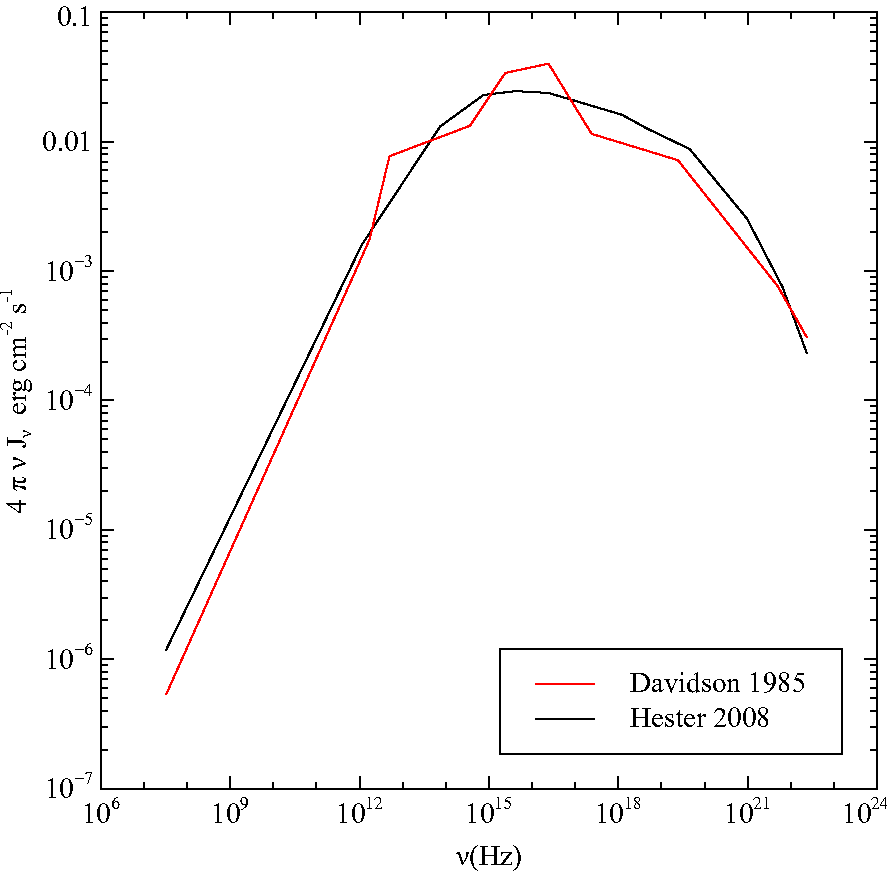
\includegraphics{CrabSED}
\caption[Crab Nebula SED]
{\label{fig:CrabSED}The SEDs produced by the \cdCommand{table Crab} 
commands are compared.
The red line is the SED from \citet{Davidson1985} and 
was the default used
by \Cloudy\ through versions C10.
The black line is the current default, derived by 
\cite{Atoyan.A96On-the-mechanisms-of-gamma-radiation-in-the-Crab}
and shown in \citet{Hester.J08The-Crab-Nebula:-An-Astrophysical-Chimera}}
\end{figure}

According to \citet{Davidson1985}, the total luminosity of the Crab is
$L_{tot} = 10^{38.14}$ \ergps.
The Crab SED could be generated by combining
the commands
\begin{verbatim}
luminosity (total) 38.14
table SED "CrabDavidson.sed"
\end{verbatim}

\subsection{Table SED ``Mrk509.sed''}

This is taken from Figure 3 of \citet{2011A&A...534A..36K}.

\subsection{Table SED ``NGC5548.sed''}

This is taken from the green line in Figure 10 of \citet{2015A&A...575A..22M}.

\subsection{Table SED ``pl1.sed''}

This produces an $f_{\nu} \propto \nu^{-1}$ power-law continuum across the
full spectral range considered by the code.
This should only be used for testing since it may produce unphysically bright 
radio or $\gamma$-ray emission.
See the discussion of the \cdCommand{power law} command on page \pageref{sec:CommandPowerLaw}
for more details, and a safe way to get a power-law continuum.

\subsection{Table SED ``Rubin.sed''}

Nearly all attempts at modeling the Orion Nebula have found that
theoretical stellar atmospheres do not produce enough flux
near 4 Ryd (see,
for example, \citealp{Mathis1982}, 1985; \citealp{Rubin1991};
\citealp{Sellmaier1996}).

Bob Rubin has modified the emergent radiation field from one of the
\citet{Kurucz1979} models to better account for the presence of
high-ionization lines in the Orion Nebula.
This modified SED can be accessed with the
\cdCommand{table SED ``Rubin.sed''} command.
The continuum started life as a
$\log g = 4$, $T_{eff} = 37{,}000$
K Kurucz model, but the flux between 41 eV and 54 eV was raised
by a factor of 11 to reproduce the [Ne III] optical and IR lines.

\subsection{Table SED ``XDR.sed''}

This generates the X-ray SED described in 
\citet{Maloney1996},
%:XDR continuum shape
\begin{equation}
f_{\nu}  = f_0 \times
\left( {\frac{{E }}{{100 \keV}}} \right)^{-0.7} 
[\ergpscmps \Hz^{-1}] ,
\end{equation}
over the energy range 1 -- 100 \keV .
The radiation field has negligible intensity outside this range.

\section{Other Table commands}

\subsection{Overview}

Any of several radiation field shapes that are stored as a permanent part
of the code can be entered with this command.
This is a special version of
the \cdCommand{interpolate} command.
The same interpolation
on a table of input frequencies and fluxes described there is done.
The \cdCommand{table} command can be freely mixed with other
shape commands and a total
of up to 100 \cdCommand{table} and \cdCommand{interpolate} commands
can be entered.

\subsection{Table AGN }
\noindent If the keyword \cdCommand{AGN} appears
(note the presence of a leading space) then
a continuum similar to that deduced by \citet{Mathews1987} will be
used.  The continuum is meant to be similar to typical radio quiet active
galaxies.
The points used to describe this continuum are given in
Table \ref{tab:AGNcontinuum}.

\begin{table}
\centering
\caption{AGN Continuum}
\begin{tabular}{lll}\hline
\label{tab:AGNcontinuum}
$\nu$(Ryd)& log $(F_\nu$)& slope\\
\hline
1.00($-$5)&$-$3.388& $+$2.50\\
9.12($-$3)&4.0115& $-$1.00\\
0.206& 2.6576& $-$0.50\\
1.743& 2.194& $-$1.00\\
4.130& 1.819& $-$3.00\\
26.84& $-$0.6192& $-$0.70\\
7.35($+$3)& $-$2.326& $-$1.67\\
7.40($+$6)& $-$7.34& $-$1.12\\
\hline
\end{tabular}
\end{table}

This radiation field differs from the \citet{Mathews1987} SED
only in that the continuum is assumed to have a sub-millimeter break at
10 microns.
For wavelengths longer than 10 microns the continuum is assumed
to have a slope $f_\nu\propto \nu^{+2.5}$,
appropriate for a self-absorbed synchrotron
continuum (\citealp{Rybicki1979}).
Note that this represents a typical
observed continuum,
and may not be directly related to the continuum actually
striking BLR gas \citep{KoristaFerlandBaldwin1997}.

The energy of the sub-millimeter break is not well determined
observationally but has a major impact on high density, high ionization
parameter models, as discussed by \citet{Ferland1989}, \citet{FerlandPeterson1992}, and \citet{Ferland1999a}.  The energy of the infrared break can be
adjusted with the \cdCommand{break} keyword.
The break can be adjusted between the
limits of 0.2 Rydberg and \emm\
by entering the keyword \cdCommand{break}
followed by a number specifying the energy of the break.  The number is
interpreted as the log of the energy in Rydbergs if it is negative and as
linear Rydbergs if positive.  It is interpreted as the linear wavelength
of the break in microns if the keyword \cdCommand{microns} also appears.
If no number appears, but the keywords \cdCommand{no break} does,
then a break at the low-energy
limit of the code (\emm ) is assumed.
The following shows
equivalent ways of generating a continuum with a break at 10 microns;
\begin{verbatim}
table AGN break .00912  # energy in Ryd
table AGN break -2.04   # log of energy in Ryd
table AGN break 10 microns # wavelength in microns
table AGN no break      # no sub-millimeter break
\end{verbatim}
Note that the nature of the SED in AGN is still an open question.  The
shape given here is very simplistic and quite uncertain in the
ionizing ultraviolet.  Moreover, it would not be surprising if the BLR
sees a far different continuum than we do.  This shape may not be
correct for low redshift Seyfert galaxies (\citealp{Binette1989};
\citealp{Clavel1990}) and direct observations of high-redshift quasars
suggest a far softer continuum than this (\citealp{Zheng1997};
\citealp{KoristaFerlandBaldwin1997}).
It is
probably best to only use this shape in exploratory situations and
generate a specific AGN radiation field using either the
\cdCommand{ratio} or \cdCommand{AGN} commands.

\subsection{Table Draine [factor=1.7]}

This enters the galactic background radiation field given by
equation 23 of \citet{Draine1996}.
The radiation field is only defined over a very
narrow wavelength range so it is only appropriate for
certain very simple PDR calculations.
It is shown in Figure \ref{fig:ISM_background} along with the
radiation field produced
by the \cdCommand{table ism} command.
This command specifies both the shape and
intensity of the continuum.

The optional scale factor changes the intensity
of the continuum.
By default it is a linear scale factor but the keyword \cdCommand{log} changes this.

This radiation field is defined up to an energy very close to 1 Rydberg.
It may spill over into the hydrogen-ionizing continuum for certain
choices of the continuum-bin resolution.
Add the \cdCommand{extinguish} command to insure that
H-ionizing radiation is extinguished if this is needed.
The code will print a comment is this is not done.

This continuum should only be used for restricted tests since the vast
majority of the electromagnetic spectrum is undefined.
It was created to compute the Leiden PDR test cases
(the \cdFilename{pdr\_leiden}* simulations in the test
suite) and the paper by \citet{Roellig2007}.

This radiation field is isotropic.
This is an intensity command.

\begin{figure}
\centering
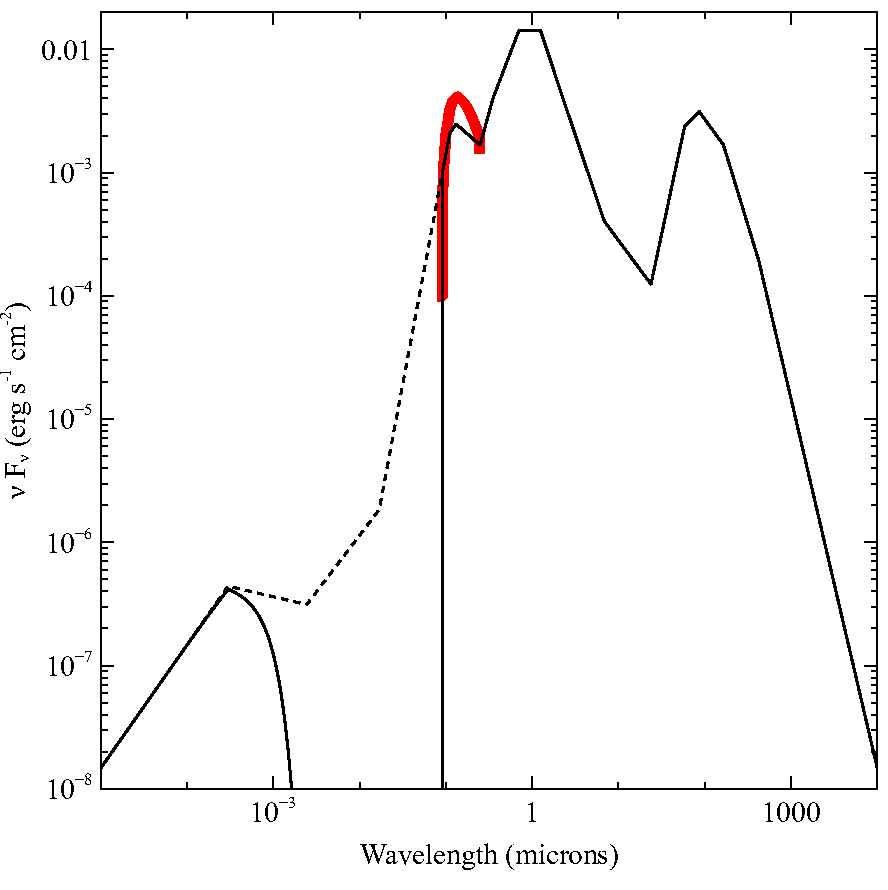
\includegraphics{ism_background}
\caption[ISM radiation field]
{\label{fig:ISM_background}The SED produced by the \cdCommand{table ISM} command is the lighter
line.
The infrared cirrus is the peak at $\lambda \sim  100\, \micron $ and starlight
dominates at shorter wavelengths.
The points just shortward of the Lyman
limit ($0.0912 \micron$) are interpolated---actually it is thought that interstellar
extinction removes most of this continuum.
The dashed line shows the
interpolated SED and the solid line shows the effects of absorption
introduced by adding the \cdCommand{extinguish} command.
The heavy red line is the \cdCommand{table Draine} continuum. }
\end{figure}

\subsection{Table HM96 [factor=-1]}

This enters the \citet{Haardt1996} background continuum for a redshift
of $z = 2.16$.  This is the original form of the command and is maintained
for reference.  The cosmic microwave background is not included - use the
\cdCommand{CMB} command to add this component.  Note that
this table specifies both the shape and intensity of the radiation field.
There
is an optional multiplicative scale factor to change the intensity.  If
the scale factor is less than or equal to zero then it is interpreted as
the log of the scale factor.

This radiation field is isotropic.
This is an intensity command.

\subsection{Table HM05 redshift 2.21 [quasar; factor=-1]}

This enters the Haardt \& Madau (2005 private communication)
radiation field at any redshift $0 \le z \le 9.479$.  It
interpolates on tables kindly provided by Francesco Haardt.  There are
two forms of the radiation field - the default includes both quasars
and galaxies.  If the keyword \cdCommand{quasar} occurs then a
radiation field considering only quasars is used.  The cosmic
microwave background is not included - use the \cdCommand{CMB} command
to add this component.  Note that this table specifies both the shape
and intensity of the radiation field.  There is an optional
multiplicative scale factor to change the intensity.  If the scale
factor is less than or equal to zero then it is interpreted as the log
of the scale factor.

The radiation field is isotropic.
This is an intensity command.

\subsection{Table HM12 redshift 2.21 [factor=-1]}

This enters the \citet{HaardtMadau2012} radiation field at any redshift $0 \le
z \le 15.93$. It works the same way as the \cdCommand{table HM05} command
described above, except that the keyword \cdCommand{quasar} is not supported
because tables for the quasar-only case do not exist for this data set.

\subsection{Table ism [factor = 0.7]}

The local interstellar radiation field is generated with the keyword
\cdCommand{ism}.
This uses Figure 2 of \citet{Black1987} to represent the
\emph{unextinguished}
local interstellar radiation field (see Figure \ref{fig:ISM_background}).  This command specifies
\emph{both} the shape and luminosity of the radiation field.
The continuum
generated by \Cloudy\ is exactly that given by Black except that the radiation
field between 1 and 4 Ryd is interpolated from the observed or inferred
values.  Actually it is thought that this part of the radiation field is
heavily absorbed by gas in the ISM so that little 1 to 4 Ryd radiation
exists, at least in the galactic plane.  Such absorption can be introduced
with the \cdCommand{extinguish} command.

The \cdCommand{table ism} command also specifies the intensity
of the incident radiation field since this is directly observed.
There is an optional scale
factor to change the intensity of the entire radiation field.
It is the
log of the scale factor if less than or equal to zero and the scale factor
itself if positive.
The actual numbers used by \Cloudy\ to interpolate on
Black's table are given in Table \ref{tab:ISM_Black}.
The frequencies are in Hz, and the
product $\nu f_\nu$ in erg cm$^{-2}$~s$^{-1}$.

This does not include the cosmic microwave background so that it can be used at any redshift.
Use the \cdCommand{CMB}
command to add this component.

\begin{table}
\centering
\caption{ISM Radiation Field}
\label{tab:ISM_Black}\begin{tabular}{llll}\hline
log($\nu$)& log $\nu f_\nu$& log $\nu$& log $\nu f_{\nu}$\\
\hline
9.00& $-$7.93& 14.14& $-$2.30\\
10.72& $-$2.96& 14.38& $-$1.79\\
11.00& $-$2.47& 14.63& $-$1.79\\
11.23& $-$2.09& 14.93& $-$2.34\\
11.47& $-$2.11& 15.08& $-$2.72\\
11.55& $-$2.34& 15.36& $-$2.55\\
11.85& $-$3.66& 15.54& $-$2.62\\
12.26& $-$2.72& 16.25& $-$5.68\\
12.54& $-$2.45& 17.09& $-$6.45\\
12.71& $-$2.57& 18.00& $-$6.30\\
13.10& $-$3.85& 23.00& $-$11.30\\
13.64& $-$3.34\\
\hline
\end{tabular}
\end{table}
The actual ISM radiation field incident on a typical region in the galactic plane could be generated by:
\begin{verbatim}
table ISM
CMB
extinguish column = 22 leak=0
\end{verbatim}

This radiation field is isotropic.
This is an intensity command.

\subsection{Table KS18 redshift 2.21 [factor=-1] [Q=18]}

This enters the \citet{KhaireSrianand2019} extragalactic background radiation
at any redshift $0 \le z \le 15$. It works very similar to the
\cdCommand{table HM12} command described above, except that there is a second
optional parameter giving the integer $Q$ parameter for the requested SED (see
Table~1 of \citealp{KhaireSrianand2019}). When omitted, it will default to
$Q18$, the fiducial model recommended by \citet{KhaireSrianand2019}. If the
$Q$ parameter is included, then adding the scaling factor is mandatory and the
scaling factor should be entered before the $Q$ parameter. Valid values for
the $Q$ parameter are between 14 and 20.

The radiation field is isotropic. This is an intensity command.

\subsection{Table power law [spectral index -1.4, low =.01, hi =20] }

This produces a power-law continuum that is well behaved at both the
high and low energy ends.
The default shape, assumed when no numbers occur
on the command line, is the form $f_\nu   \propto \nu ^\alpha  $.
Here
$\alpha = -1$ for the spectral midrange between 10 microns and 50 keV,
and the continuum has slopes $f_\nu   \propto \nu ^{5/2} $ at lower energies (appropriate for self-absorbed synchrotron, eq 6.54,
p.190, \citealp{Rybicki1979}) and
$f_\nu   \propto \nu ^{ - 2} $ at higher energies.
Note that much of the X-ray literature will use
an implicit negative sign in defining the energy index,
as in equation 13.2 of AGN3.
\Cloudy\ never uses implicit negative signs so a typical AGN will
have an energy index of roughly $-$1.5.
Table \ref{tab:PowerLawContinuum} summarizes the continuum
that is produced by this command if no other parameters are specified.

\begin{table}
\centering
\caption{Power Law Continuum}
\begin{tabular}{ll}\hline
\label{tab:PowerLawContinuum}
$\nu$(Ryd)& slope\\
\hline
1.00($-$8)& $+$2.50\\
9.115($-$3)& $-$1.00\\
3676.& $-$2.\\
7.40($+$6)& $-$\\
\hline
\end{tabular}
\end{table}

Three optional numbers may appear on the command line.
The first number
sets the slope of the mid-range spectral component (infrared to X-ray)
and has a default of -1 ($f_\nu   \propto \nu ^{ - 1} $).
The
next two numbers adjust the energy limits of the mid-range spectral
component.
Their default units are Rydbergs but the keyword \cdCommand{microns} will
change the units to microns \emph{for the first energy only.}
The second number
is the energy (in Rydbergs) of the infrared break.
The default is 0.009115
Ryd (10 microns).
If this second number is zero then the low energy limit
to the continuum (\emm ) will be used.
The number is interpreted
as the log of the energy in Rydbergs if it is negative and linear otherwise.
Note that, with no infrared break, free-free heating will probably be
significant for denser clouds.  A power-law continuum with a low energy
break at 1 micron would minimize this heating and could be generated with
the command
\begin{verbatim}
# a power-law with index -1 and 1 micron break
table power law slope -1, 1 micron break
\end{verbatim}
The following uses the default power law
\begin{verbatim}
# another example, a power-law with index -1
# and 10 micron break, (the default)
table power law slope -1
\end{verbatim}

The third optional number is the energy (in Rydbergs) of the break in
the X-ray continuum.
The default is 50 keV and if it is zero then the
high-energy limit of the continuum (\egamry ) is used.
The number is interpreted as a log if the energy of the
infrared break is entered as
a log and linear otherwise.
The numbers may be omitted from right to left.

\subsection{Table read "contin.txt" [ scale [ = 0.5 ] ]}
\label{sec:CommandTableRead}

This reads in the radiation field predicted from
a previous \Cloudy\ calculation.
The name of the file containing the spectrum predicted
from the first calculation continuum must be enclosed
in a pair of double quotes.
The first calculation saves the radiation
transmitted through a cloud with the
\cdCommand{save transmitted continuum} command described in Section
\ref{sec:CommandSaveTransmittedContinuum}.
Subsequent calculations use the \cdCommand{table read} command
to include this field.

The transmitted spectrum of the first model
will include all transmitted radiation, including line emission, and
will write that out as a single spectral energy distribution. When the
second model reads that in, it will have no knowledge of what was what
in the first model, apart from the outer radius of that model
(assuming a radius was specified in that model).
It will treat it as an incident SED without further
specifics. So the [\oiii ] 5006.84 flux reported by the second model will be
that produced by the second model only, but the 5006.84 photons from the
first model will be included ``anonymously'' in the incident SED.

The \cdCommand{save transmitted continuum} command produces a file containing the frequency in Rydbergs and the transmitted
continuum $\nu f_{\nu}$ [erg cm$^{-2}$ s$^{-1}$].
This continuum is the sum of the attenuated
incident continuum and the fraction of the cloud's diffuse emission
that is transmitted in the outward direction.  The first lines of the 
file contain header information and must not be deleted.

\Cloudy\ checks that the photon energies contained in the
\cdCommand{save transmitted continuum} file are exactly that same as
the photon energies used in the code's internal arrays.  
This is because the contents of the files are simply placed into these arrays with
no interpolation.  You should not try to change the photon energies.

The \cdCommand{table read} command can be freely mixed with all
of the other radiation field shape commands.
Any number of \cdCommand{table read} commands can be entered.\footnote{Only one table read command could be entered in versions
90 and before.}
The \cdCommand{save continuum} file must have been produced by the same version of \Cloudy.

By default, this command does not set the intensity of the radiation
field.  If the \cdCommand{scale} option is not given, the intensity of the
radiation field must be set explicitly, using any of the intensity or
luminosity commands.

If the \cdCommand{scale} option is given, the
intensity scale can be specified relative to the intensity of the previous
calculation.  As with some other \cdCommand{table} commands, the value
specified is interpreted as a log scale if it is non-positive and linear
otherwise. If no number is given, the scale factor defaults to unity.

If the model that generated the transmitted spectrum and the model that reads
it both set a radius, then spherical dilution will implicitly be done. The
scale factor will be a multiplicative factor on top of that, i.e. the
transmitted spectrum will be multiplied by a factor $(r_{\rm out}/r_{\rm
  in})^2 s$ where $r_{\rm out}$ is the outer radius of the first model,
$r_{\rm in}$ is the inner radius of the second model, and $s$ is the scale
factor. A warning will be printed if $r_{\rm in} < r_{\rm out}$, but the
spherical correction will still be done (which would make the radiation field
more intense). If the first model set a radius, but not the second (or {\it
  vice versa}) a caution will be printed and no spherical correction will be
done (but the scale factor will still be applied).

The following gives an example of first creating a file containing the
transmitted radiation field then using this file as the
incident radiation field in a second calculation.
\begin{verbatim}
title this finds transmitted continuum due to warm absorber
hden 9
ionization parameter 1
stop effective column density 21
table AGN
iterate
save transmitted continuum file = "absorber.txt" last
\end{verbatim}
Now use this continuum in a second calculation:
\begin{verbatim}
table read file = "absorber.txt"
luminosity 45
radius 18
hden 9
\end{verbatim}
The output continuum can also be diluted by a factor of 100 compared
to the first calculation:
\begin{verbatim}
table read file = "absorber.txt" scale -2
hden 9
\end{verbatim}

\subsection{Table trapezium}
\label{sec:CommandTableTrapezium}

This enters the radiation field of the Orion Trapezium stars.


\section{Table stars command}
\label{sect:TableStars}

Several sets of emergent SEDs from stellar atmosphere calculations are
accessible.
The command has several sub-keywords that indicate which set
of atmospheres to use. The syntax of the command varies depending on
how the atmosphere grid was constructed. The easiest way to find out
how to use this command is by entering the command \cdCommand{table
star available} after the grids have been installed. The 
\cdCommand{table star} accepts the optional keyword \cdCommand{log}
which indicates that the first number on the line is the logarithm of
that parameter. Usually that is the effective temperature.

Figure \ref{fig:StarsContinuum} compares predictions for
five of the 50~kK SEDs that are
available.  These include a blackbody and atmospheres computed by \citet{Mihalas1972}, \citet{Kurucz1979}, \citet{Kurucz1991} and \citet{Rauch2002}.
All were normalized
to have the same total luminosity ($10^{38}$ erg s$^{-1}$)
observed from a distance of $10^{18}$~cm.
Note the order of magnitude dispersion among the continua for
energies around 4 Ryd.

\begin{figure}
\centering
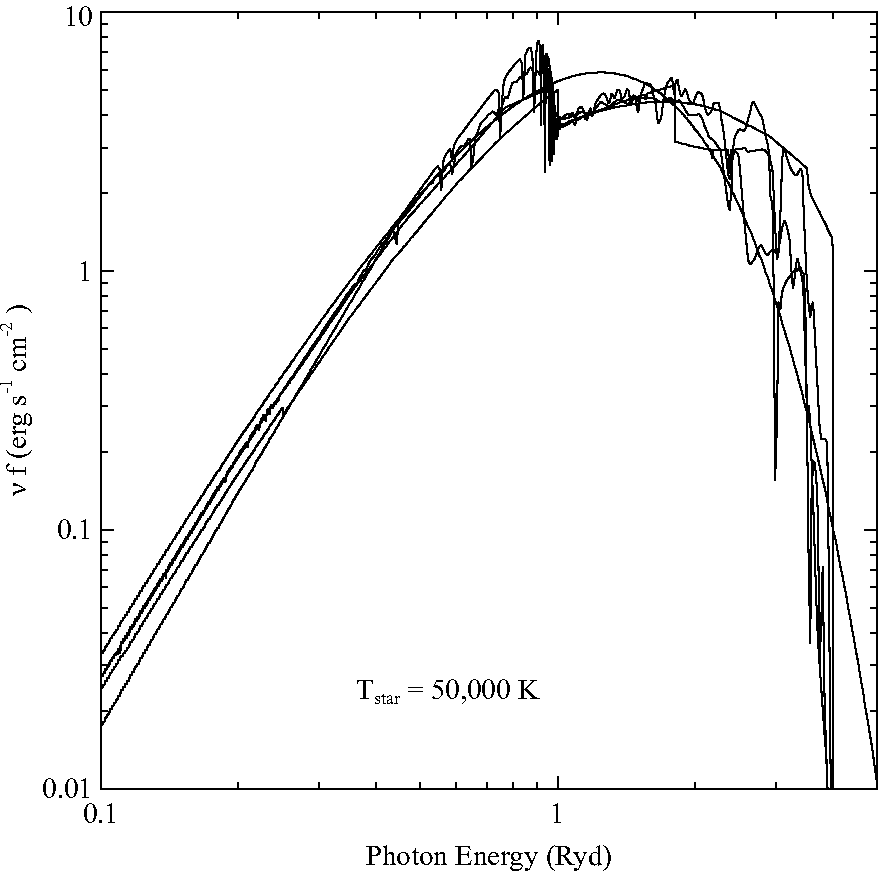
\includegraphics[scale=0.9]{StarsContinuum}
\caption[Stellar radiation fields]
{\label{fig:StarsContinuum}This figure shows the emergent
radiation field predicted by five 50~kK 
stars included with the code.  The smoothest is the blackbody, and the
\citet{Kurucz1991} and \citet{Rauch1997} atmospheres show the most structure.  stars}
\end{figure}

These commands specify only the continuum shape.
It is still necessary to specify a luminosity.
\citet{Tout1996} provide convenient fitting
formulae giving zero age main sequence luminosities as
functions of stellar mass and metallicity.

{\bf Danger!}  Many forms of the \cdCommand{table stars} commands
accept the \cdCommand{log} keyword to indicate that the log of the stellar temperature
is entered.  Many also accept the surface gravity, normally referred to as
``log g'', as a second parameter.  The ``log'' in ``log g'' would cause the
temperature to be interpreted as the log of the temperature.  Either
do not enter the string ``log g'', or write it as ``logg'' or ``log(g)''.

\subsection{Overview of available stellar SEDs}

In versions C06.02 and before the stellar continua were entered into
the code on a case by case basis.
New continua could only be introduced
by writing new code.
Beginning in C07.02 Peter van Hoof developed a unified
treatment so that any continuum could be used by putting
it into a standard format.
This is far more flexible and allows more continua to be entered.

Usually grids have a range of surface temperature, and many also include a
range of surface gravity or metallicity. But other types of parameters are
also possible, e.g., age in the case of stellar population synthesis models.
The \cdCommand{table star} command will interpolate on these tables to
calculate an SED with the specified parameters. More information on the
various grids that are supported can be found on our web site
\href{http://wiki.nublado.org/wiki/StellarAtmospheres}{wiki.nublado.org/wiki/StellarAtmospheres}.

To list all the grids that have already been installed on your system, you can
use the \cdCommand{table star available} command. This will list all the
standard grids that were installed from the webpage above (including their
parameters), but not the custom grids that you created yourself.
The output will also list the \cdCommand{table HM05}
and \cdCommand{table HM12} commands. They are not strictly part of the
\cdCommand{table star} family of commands, but they internally use the stellar
grid infrastructure to do their work.

To list all the SEDs that are contained in a single stellar atmosphere
grid, you can use the \cdCommand{table star $<$grid$>$ list} command. For more
details see our webpage listed above.

\subsection{High-energy component}
\label{sec:StarHighEnergyComponent}

Theoretical stellar atmospheres emit little energy above 4 Ryd while
real OB stars \emph{are} X-ray sources.
\citet{Sciortino1990} find a correlation
between the X-ray and bolometric luminosities which can be fitted~by
\begin{equation}
\log \left( {L_x } \right) = 1.08\left( { + 0.06/ - 0.22} \right)\,\log
\left( {L_{bol} } \right) - 9.38\left( { + 2.32/ - 0.83} \right) .% (25)
\end{equation}
The X-ray luminosity is typically $\sim 6.4$ dex fainter
than the bolometric luminosity.
A source temperature of 0.5 keV is quoted by Sciortino et al.
This X-ray component must be explicitly added as an
independent part of the incident radiation field.
Tests show that the high-energy light has little effect on
conditions in the H~II region but \emph{does} affect the
ionization in the surrounding PDR.

\subsection{Starburst99 files}

It is possible to read in predictions from Starburst99 
(\citealp{Leitherer1999}).\footnote{The \cdCommand{table starburst} command, 
which existed for this purpose in versions through C07, has been replaced
with this  \cdCommand{table stars} command.}
The Starburst99 SEDs are unified with the stellar
atmosphere treatment.
See our web site
\href{http://wiki.nublado.org/wiki/StellarAtmospheres}{wiki.nublado.org/wiki/StellarAtmospheres} and
Appendix~\ref{ascii} below for more details.

The procedure is to create your Starburst99 calculation on their web site
(we tested the version at STScI).
Store the Starburst99 output file ``*.spectrum1'' as
a file with a ``\cdFilename{.stb99}''  or ``\cdFilename{.stb}'' extension.
Compile it as in the following example
\begin{verbatim}
compile star "some_file.stb99"
\end{verbatim}
You can optionally include the keyword \cdCommand{stellar} or
\cdCommand{nebular} if you want to use only the stellar or the nebular
component of the interstellar radiation field (these are the fourth and fifth
column of the Starburst99 calculation, respectively). The default is to use
the total spectrum, which is the sum of the stellar and nebular component.
This would be the equivalent of including the emission from nearby star
forming regions in your calculation. If you don't want that, you can use the
stellar component only, as in the following example
\begin{verbatim}
compile star "some_file.stb99" stellar
\end{verbatim}
The above commands will produce files \cdFilename{some\_file.ascii} and
\cdFilename{some\_file.idx}, which can then
be used in the \cdCommand{table stars} command:
\begin{verbatim}
table star "some_file.ascii" age=6e7 years
\end{verbatim}

The number on the \cdCommand{table star} command is the
age of the starburst.  It has the same units as the ages given in the
Starburst99 data file and is normally given in years.
It is interpreted as a log if the keyword \cdCommand{log} appears,
and as the linear age otherwise.

It is critical that the original Starburst99 file not be
changed in any way at all.
Doing so will trick the code into generating bogus results.
In any case, it is a good idea to make a plot of the generated
radiation field,
using column 1 and 2 of the output from
the \cdCommand{save continuum} command, to confirm that it is correct.

Starting with the C10 release it is possible to combine several
Starburst99 runs with different metallicities into a single 2-dimensional
grid. This allows interpolation in both age and $\log Z$. This has
to be done by compiling each of the Starburst99 runs as described above
and then manually merging the ``\cdFilename{.ascii}'' files into a single
``\cdFilename{.ascii}'' file. Appendix~\ref{ascii} gives details how the merged
file should be formatted. An example of a merged file is available on the
StellarAtmospheres page of the Cloudy wiki linked at the start of this subsection.
The resulting file can be compiled using
\begin{verbatim}
compile star "merged_file.ascii"
\end{verbatim}
and used as follows
\begin{verbatim}
table star "merged_file.ascii" age=6.7 log(Z)=-1.2
\end{verbatim}

\subsection{PopStar and BPASS grids}

You can convert PopStar and BPASS grids into ``\cdFilename{.ascii}'' files so
that they can be used in \Cloudy. You can either use a single PopStar grid,
allowing interpolation in age, or combine several PopStar grids for the same
initial mass function but different metallicities allowing interpolation in
age as well as $\log Z$. Detailed instructions can be found on
\href{http://wiki.nublado.org/wiki/StellarAtmospheres}{wiki.nublado.org/wiki/StellarAtmospheres}.
